\documentclass[12pt,a4paper]{article}
\usepackage[a4paper,top=1in,bottom=1in,left=1.25in,right=1.25in]{geometry}
\usepackage{amsmath,latexsym,amssymb,stmaryrd}
\usepackage{amsfonts,amsthm}
\usepackage[utf8]{inputenc}
\usepackage[OT1]{fontenc}
\usepackage[french]{babel} % important pour la typographie et les césures
\usepackage{verbatim,alltt,bm}
\usepackage{xcolor}
\usepackage{tikz}
\usetikzlibrary{arrows,shapes}
\usepackage{hyperref}
\usepackage{fancyhdr}
\usepackage[myheadings]{fullpage}
\setlength{\topmargin}{-1cm}
\setlength{\textheight}{25cm}
\usepackage[linewidth=1pt]{mdframed}
\usepackage[section]{placeins}
\usepackage{graphicx}
\usepackage{subfigure}
\usepackage[titletoc]{appendix}
\usepackage[figuresright]{rotating}


\title{Acoustic Keylogger}
\author{\\\\\\\\\\\\\\\\\\HAN Xicun\\\\
Director : Christophe. Rosenberger\\\\
Informatique M2 , Science\\\\
University of CAEN \\\\
\texttt{xicun.han@gmail.com}\\\\}
\date{24 February 2017}



\begin{document}
	\pagestyle{empty}
	\maketitle
	\thispagestyle{empty}
	\clearpage
	%\pagebreak
	
	
	\tableofcontents
	
	\thispagestyle{empty}
	\newpage
	\pagestyle{fancy}
	\lhead{}                    
	\chead{}                                                
	%\rhead{}  
	%\begin{abstract} \setcounter{page}{1}
	%	Ã  remplir
	%\end{abstract}
	\pagebreak
	\FloatBarrier

\begin{abstract}

When assessing the security of security systems, it is fatal to take a consideration of conceptual new attacks, as countermeasures nowadays can only be implemented against known threats. With this consideration, in this report, we are going to explore the acoustic side channel attack and evaluate each one. \\

In this report we are going to review the related works and bring analysis to the characteristics of each one,  and at last perform a empirical study of one approach.\\


\end{abstract}
\newpage


\section{Introduction}

Nowadays, password is still performing an important role in our daily authentication process. It has been used as a primary means to get access to the Internet resources, the sensitive user data or even more to the banking payment process.  \\

As most of the authentication method, it is now facing a verity of security problems, such as brute-force attack, key logger, vibration side channel attack, timing attack, electromagnetic radiation attack etc. In this paper we will focus on the empirical implementation of the acoustic side channel attack with different strategies.\\

\subsection{Password and Related Security Issues }

The password, as we mentioned, is used with an identity to gain access to certain resources, and its security is often questioned. It has been proved to be weak against brute force attacks, keyloggers as well as side channel attacks. \\

A brute force attack can be easily performed by trying each possible combination of alphabets, since a user is often in the habit of putting his or her personal information into the password and moreover keeping it short so that he / she can easily remember, this classical method is sometimes very effective. \\

A keylogger can be a malware in the system or hardware memories the typing of user.\\

\textbf{Side channel attack} on the other hand, is harder to detect and defend, because it measures the implementation of an algorithm beyond the algorithm itself. For example, timing attack through the internet measures the reacting-time of IP package, the power monitoring attack measures the power consuming during each computation. In this project we will analyses the acoustic side channel attack. \\


\subsection{Acoustic Side Channel Attack}

\textbf{The acoustic side channel attack} is based on the acoustic emanations produced by electronic devices such as a US-101 standard keyboard or a specified keyboard used by Bank, the conspicuous sounds produced by typing can be used to learn information about the input data. \\

Recent studies utilize a variety of methods in order to capture the features of one's in order to lance this type of attack.\\



\newpage

\section{Related Works Overview}


\textbf{Asonov and Agrawal\cite{DBLP:conf/sp/AsonovA04}} were the first researchers to demonstrate the threat of side channel attacks using acoustic leakage from the keyboard. They used the Fast Fourier Transform (FFT) features of the extracted keystroke as an identifier and use a neural network to classify and recognize the keystrokes. This process involved a training phase that used labeled data pair consisting of a key and its corresponding feature, and a testing phase that took a feature as an input and the output consisted of the closest matching key.\\

\textbf{Zhuang et. al\cite{DBLP:conf/ccs/ZhuangZT05}}. extended the work of Asonov and Agrawal by using cepstrum features, in particular Mel-Frequency Cepstrum Coefficients (MFCC) as identifiers for the keystrokes and used unlabeled data in the training phase for the neural network unlike Asonov and Agrawal.\\

\textbf{Berger et al.\cite{DBLP:conf/ccs/BergerWY06}}  used cross correlation between the recorded keystroke signals and euclidean distance between frequency based features to classify and recognize the keystrokes. They then used dictionary based attack to reconstruct the text from the recovered keystrokes.\\

\textbf{Halevi and Saxena\cite{DBLP:conf/ccs/HaleviS12}} combined the cross correlation information between the two keystrokes signals and the frequency distance measure from the work done by Berger et al. to create a new feature called time-frequency classification. This new feature was used for identifying different keystrokes and then used for password detection. They also studied the effect of various typing styles (hunt and peck, and touch typing) on keystroke signal similarities and found out that the signal similarity decreases with change in the typing style.\\

\textbf{Fiona\cite{Fiona2006}} presented a distance-time based triangulation attack that is able to identify a keystroke by recording the keystroke with multiple microphones. Due to fixed location of each key on the keyboard, the sound recorded by each microphone arrives at a different time and the time delay for each keystroke can be used to distinguish between the keystrokes\\




\subsection{Asonov and Agrawal}

In 2004, at the very beginning, the keyboard acoustic emanations was recognized as a threat by Dmitri Asonov and Rakesh Agrawal from IBM  Almaden Research Center in their paper. \\

The basic idea is the assumption that the sound of clicks differ slightly from one key to another. In this way,  features can be extracted from these different sound of keystrokes. \\

Their methodology:
\begin{itemize}
\item[•] The press and release action produced different sounds. It is found that knocking at different parts of a mechanical keyboard plate produce different sounds. It is like striking at the different locations of a drum will produce different sounds.\\
\item[•] Within the sounds of thirty keys of a single PC keyboard they recorded, they found out that the Fast Fourier Transform values of the press peaks give significant variation for perceptually similar sounds.\\
\item[•] The frequency distributions were passed into a neural network for classification.  The neural network was trained with pairs \{key, feature\}\\
\end{itemize}

\begin{figure}[h]
\begin{center}
        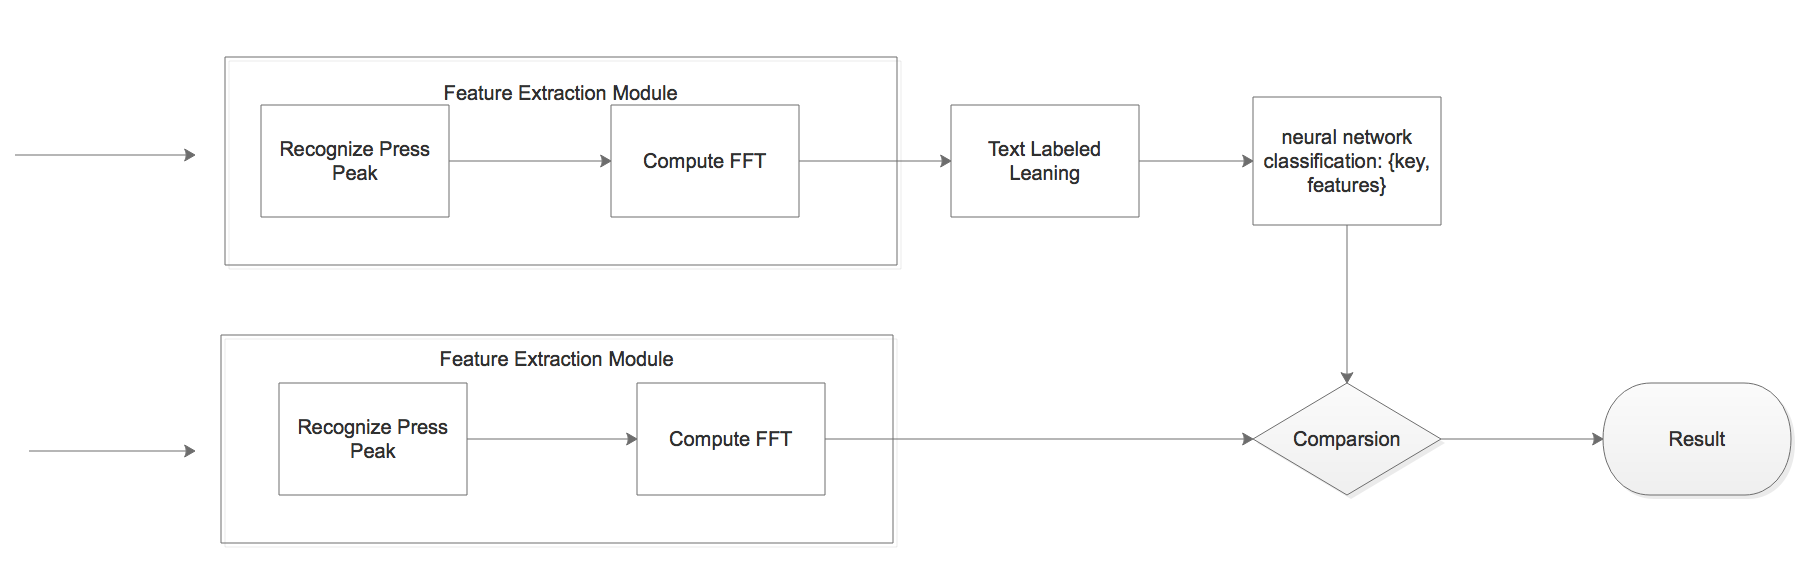
\includegraphics[scale=0.55]{aaModel.png}
        \caption{The Asonov and Agrawal proposal}
        \label{fig:3}
\end{center}
\end{figure} \par
\FloatBarrier

Through experimenting with several sets of data, the best recognition rate can be achieved by including the entire active interval in the feature extraction, the 300-3400 Hz interval is approved to be the most informative.\\

The accuracy rate for a key to be recognized correctly is approximately 80\%. Besides the facts that different keyboards produce different sounds, the sound for each key is unique, theoretically, the keys can be recognized regardless of the keyboard type and the typing style, but as their experiment is held by one person, the performance would have been affected if they would have tried to recognize the typed keys on a different key board and with another tying style.\\

\subsection{Zhuang et. al}

From the previous introduction to Asonove and Agrawal's attack, we recognize immediately the limit of this model. Their attack requires neural network training with text-labeled samples, and for the most of the time in reality, the training sample of a significant length is difficult to obtain.\\ 

Zhuang Zhou and al. published another proposal which is developed by Zhuang, F.Zhou and J.D.Tygar in the year 2005. They argue that a labeled training sample requirement is unnecessary for an attacker, as they mentioned in their paper "\textit{The key insight in our work is that the typed text is often not random, when one types English text, the limited number of English words limits the possible temporal combinations of keys, and the English grammar limits the word combinations.}" This fact makes the keyboard emanation attacks a more serious security problem.\\

Given the ideal assumption that each key sounds exactly the same then it is pressed,  then the problem can be considered as a machine learning version of substitution ciphers. The Figure ~\ref{fig:4} captures an overview of their approach.  \\


\begin{figure}[h]
\begin{center}
        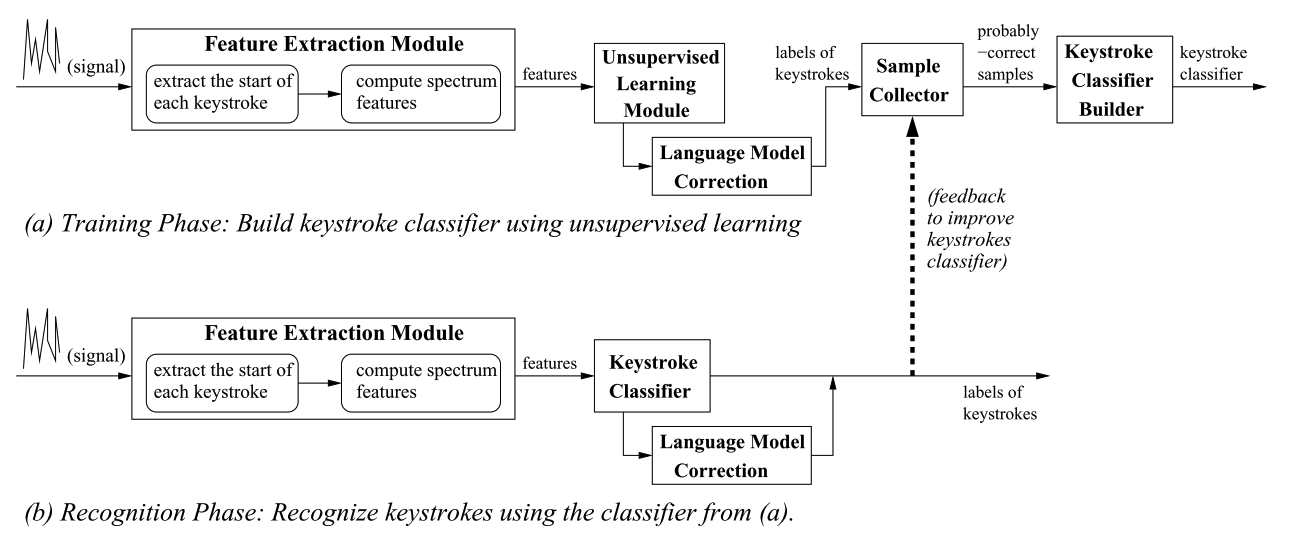
\includegraphics[scale=0.38]{zhuangModel.png}
        \caption{Over View of the  Zhuang Zhou Tygar Model}
        \label{fig:4}
\end{center}
\end{figure} \par
\FloatBarrier 

\subsubsection*{Keystroke Recognizing}
\begin{figure}[h]
\begin{center}
        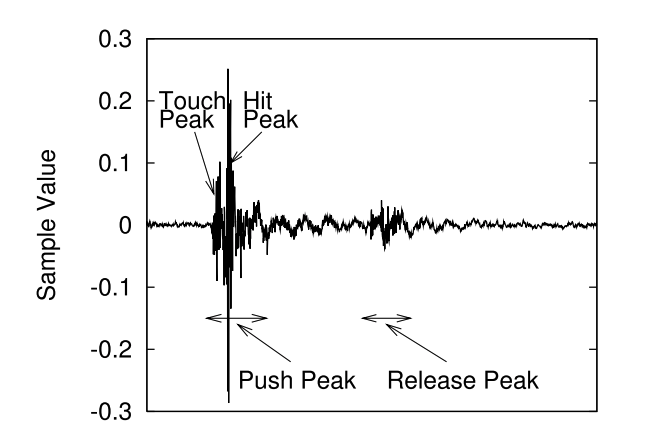
\includegraphics[scale=0.45]{audioSignal.png}
        \caption{The audio signal of a key stroke}
        \label{fig:1}
\end{center}
\end{figure} \par
\FloatBarrier

As shown in Figure ~\ref{fig:1}, a keystroke consists a push and a release actions which can be easily observed. Studies of Asonove and Agrawal have shown that the period from push to release is typically about 100 milliseconds\cite{Gould2005}. The fact to have more than 100 milliseconds between consecutive key strokes allows us to distinguish the consecutive keystrokes and find the beginning for each window as it is shown in Figure ~\ref{fig:2}. They calculate windowed discrete Fourier transform of the signal and use the sum of all FFT coefficients as energy, then use a threshold to detect the start of each one.\\

\begin{figure}[h]
\begin{center}
        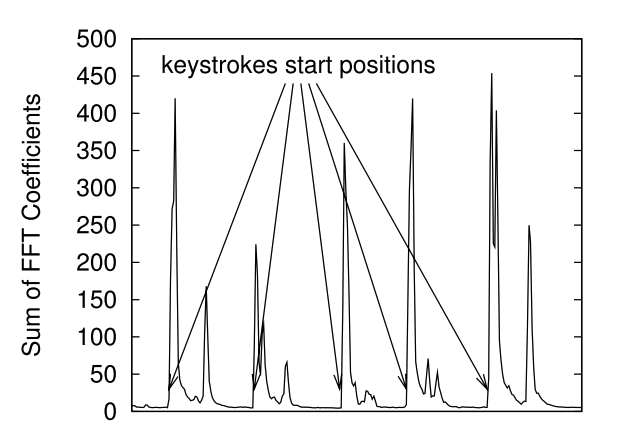
\includegraphics[scale=0.45]{energyLevel.png}
        \caption{Energy levels over the duration of 5 keystrokes}
        \label{fig:2}
\end{center}
\end{figure} \par
\FloatBarrier

\subsubsection{Cepstrum features extraction}
In the part of feature extraction, in their paper, it has been proved that the Cepstrum features which is widely used in speech analysis and recognition has empirically higher performance than the plain FFT coefficients, In particular, they used Mel-Frequency Cepstral Coefficients (MFCCs) in the experiments.

\subsubsection{Unsupervised key recognition}

As we discussed before, our ideal aim is to build an one-to-one mapping between the keys and classes. however, as the variability of the situation, one key stroke can be in different classes, at the same time, one class can contain several keystrokes. In the end, a particular key will be in each class with a certain probability.\\

The next work is trying is trying to find the sequence of keystrokes based on a sequence of classes for each keystroke. A \textbf{HMM(Hidden Markov Models) algorithm} will be served for this prediction.\\

In a hidden Markov model, the state is not directly visible, but the output, dependent on the state, is visible. Each state has a probability distribution over the possible output tokens. Therefore, the sequence of tokens generated by an HMM gives some information about the sequence of states. The adjective 'hidden' refers to the state sequence through which the model passes, not to the parameters of the model; the model is still referred to as a 'hidden' Markov model even if these parameters are known exactly.\\

For example, if the current key can be either “h” or “j” (e.g. because they are physically close on the key- board) and we know the previous key is “t”, then the current key is more likely to be “h” because “th” is more common than “tj”.\\

\subsubsection{Spelling and Grammar Checking}
In the work of Zhuang Zhou et Tygar, they implemented:\\
\begin{itemize}
\item[•] A dictionary based spelling correction
\item[•] A simple static model of English grammar.
\end{itemize}

\subsubsection{Feedback based training}

Feedback training procedure will not use the English spelling and grammar model in order to detect a password. The previously obtained corrected results is used as a labeled training samples. In this way a circle is formed, and the spelling and grammar correction, on the other hand is used as a quality indicator. The same feedback procedure is done repeatedly until no significant improvement is seen. \\
 
\subsection{Berger et al.}

Yigael Berger, Avishai Wool and ArieYeredor (Berger, et al., 2006) present a dictionary attack based on their previous research, this attack does not require any training and works on  an individual recording of typed word and is efficient for the short patterns which we always chose as password.\\

This attack is made up from several steps: \\
\begin{itemize}
\item[•] Signal Processing and Feature Extraction
\item[•] Keystroke Processing
\item[•] Constraint Formulation 
\item[•] Constraint Evaluation
\item[•] Outcome Prioritization
\end{itemize}

\subsubsection{Signal Processing}

As we mentioned before, the keystroke is consist of the action of PRESS and the action of RELEASE. The out put of this part should be two arrays of signal segments consist $PRESS_{i}$ and $RELEASE_{i}$ separately.\\

\subsubsection{Keystroke Processing}

Our goal is always seeking for a metrics $sim(K_{1},K_{2})$ which will allow us to distinguish two keystrokes, and particularly in this part, they aimed at finding a metrics that will represent the keys' physical proximity on the keyboard. \\

\begin{figure}[h]
\begin{center}
        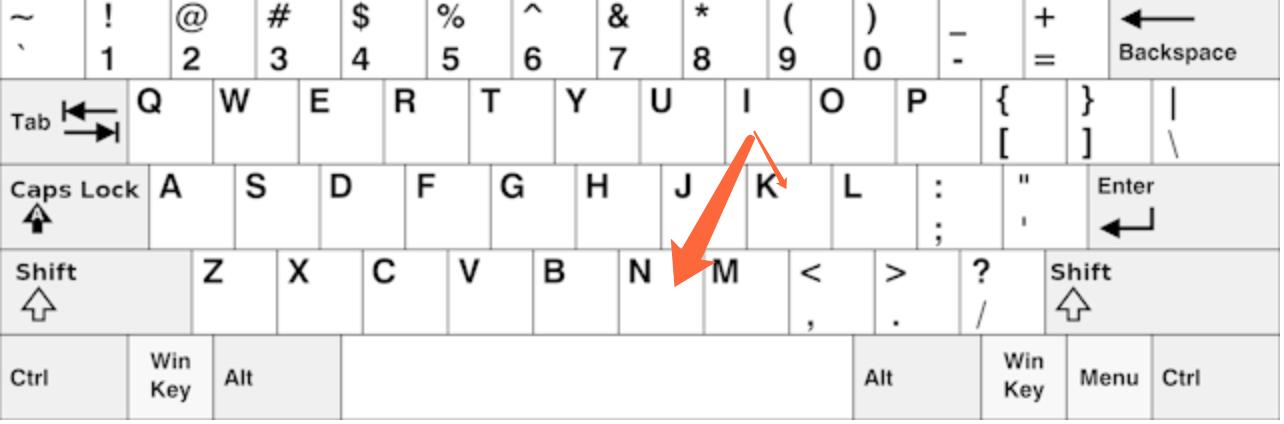
\includegraphics[scale=0.45]{keyboardQwer.png}
        \caption{Physical Proximity Measure}
        \label{fig:5}
\end{center}
\end{figure} \par
\FloatBarrier

That is to say, as shown in Figure ~\ref{fig:5}, $sim(K_{i},K_{k})<sim(K_{i},K_{n})$ implicate the physical distance between key i and key n is further than that between key i and key k. For this propose the most adaptive metric is the cross-correlation metric who has a even better performance than fft and Cepstrum.\\

In this way, we calculate the $sim(K_{1},K_{2})$ for each $PRESS_{i}$ to every other press and the same with each $RELEASE_{i}$. After the calculation we will have two matrix the $N*N$. In the end, they found out that an unweighted average method perform good in combining the Press Similarities with the Release Similarities.\\ 

\subsubsection{Constraint Formulation}

With the function $sim(K_{1},K_{2})$ whom we calculate the distance, 4 kinds of relations between two keys are defined : 
\begin{figure}[h]
\begin{center}
        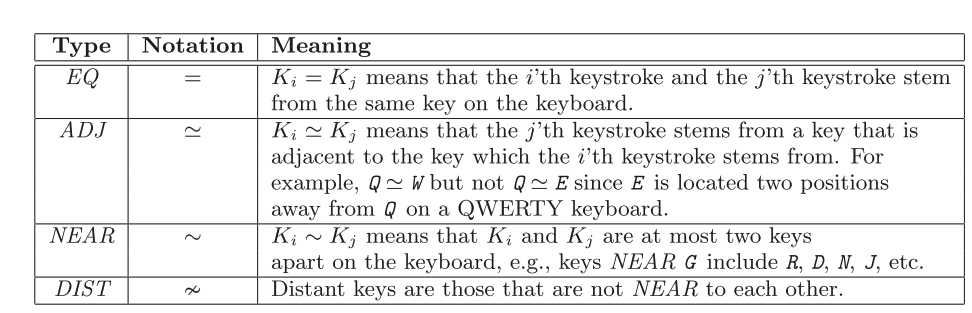
\includegraphics[scale=0.45]{4ConstraintTypes.png}
        \caption{The 4 Constraint types}
        \label{fig:6}
\end{center}
\end{figure} \par
\FloatBarrier

A word will produces a set of constraints, but a sequence of constrains corresponds to several different sets of word. For example, the word "help" in a QWER keyboard produces the following constrains: (DIST$<1,2>$, DIST$<1,3>$, DIST$<1,4>$, DIST$<2,3>$, DIST$<2,4>$, ADJ$<3,4>$ ). Meanwhile, we will find that "nose", "path" etc. have exactly the same combination. \\

\subsubsection{Constraint Evaluation}

The process of evaluation is based on the assumption that we know the length of the word N,  what we will do is to go over all permutation the words of length N and output all those who match the constraints.\\

They also use some measures to reduce the errors, for the reason that if in the sequence of constraints, there's an error happened, we will never get the good response. For this purpose, two metrics for each constraint type are implicated:\\
 
\begin{itemize}
\item[•] Precision :True positives/Total number of positives predicted  =  TP/(TP+FP)
\item[•] Recall :  True positives/Total number of actual positives = TP/(TP + FN)\\
\end{itemize}

And in order to get the best combination, they came up with the idea of \textit{BestFriendsPickPolicy} with which we can generate the possible arrangement based on the physical positions of each key on the keyboard.\\

 \subsubsection{Dealing with False Constraints}
 
Given that all we have argued are true, after the evaluation, many combinations will be consistent with the correct word. However, this method will produce eventually the possible combinations which is explosive.  So as to overcome this explosion, they empirically found that 1000 random chosen combinations are usually suffice, then for each combination c, c is evaluated against the possible words in the dictionary. As an output, we will have $L_{c}$ that conform with the selected constraints of combination c.\\

\subsubsection{Outcome Prioritization}

Based on $L_{c}$ lists, For each word w in the dictionary we count the number of combinations c for which $w \in L_{c}$ and sort the words in decreasing order and after trying enough combinations the correct word will appear near the top of the sorted unified list.  \\


\subsection{Halevi and Saxena}

As we discussed, The study of Halevi and Saxena brings optimization above the Detection techniques and analyze the influence of user typing styles.\\

\subsubsection{Time-frequency Classification}
\newcommand{\tabincell}[2]{\begin{tabular}{@{}#1@{}}#2\end{tabular}}  

We have already discussed several technologies of detection of signal: \\


\begin{tabular}{| l | l | }
\hline Technique & description \\
\hline Dynamic Time Warping & \tabincell{l}{an algorithm which measures the similarities between sequences\\
(calculate the simple distance measure between two signal vectors)\\
Usage: \\
- Collect Letter Date Set\{key, samples\} \\
- Compare to get best match } \\

\hline Cross-Correlation & \tabincell{l}{ Algorithm measures the similarity :\\
- Signal normalized according to their energy\\
- calculated for the press and release regions.\\
Usage: \\
- Construct Letter Data Set\\
- Calculate the average of their Cross-correlation measurement\\
- find matches with the highest similarity.}\\

\hline \tabincell{l}{ Frequency-based \\ Distance Measure} & \tabincell{l}{Algorithm measures the similarity :\\
- calculate Euclidean difference for PRESS and RELEASE parts\\
- calculate Average as a distance measure\\
Usage: \\
- calculate the distance between each test sample and each letter \\Data Set \\
- output the letter with the smallest distance. }\\

\hline \tabincell{l}{ Frequency Features and \\ Neural Networks} & \tabincell{l}{
implement the frequency-domain features, \\ using MFCC features as input to neural networks. }\\
\hline
\end{tabular}\\\\

With an empirical evaluation, a table of detection rate out of 26 alphabet letters is constructed as shown in the Figure ~\ref{fig:7}, from their observation, the Cross-Correlation has a relatively high score, and when they combined the correlation calculation with the frequency based calculations to choose the best-matching letter, they got a even higher score and the named it "Time-Frequency Classification". \\

\begin{figure}[h]
\begin{center}
        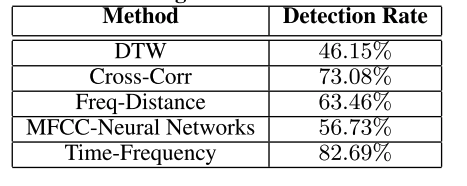
\includegraphics[scale=0.5]{singleCharDetectionPerfo.png}
        \caption{Single Character Detection}
        \label{fig:7}
\end{center}
\end{figure} \par
\FloatBarrier

\newpage


As described in Figure ~\ref{fig:8}, in the time frequency classification method. Firstly we calculate the Cross-Correlation denote F and the Frequency Distance denote C from the instance. Then, for the purpose of having the same ascending order, DC is calculated from C where $DC_{i} = 1-C_{i}$. \\

In order to combine two factors, we have a lot of proposals: 
\begin{itemize}
\item[•] Picking the minimum of each value (min(DC,F))
\item[•] Getting the average of the two values:  Mean(DC,F)
\item[•] Considering (F,DC) as a point on a 2-D space and calculate the Euclidean distance from zero\\
\end{itemize}
\begin{figure}[h]
\begin{center}
        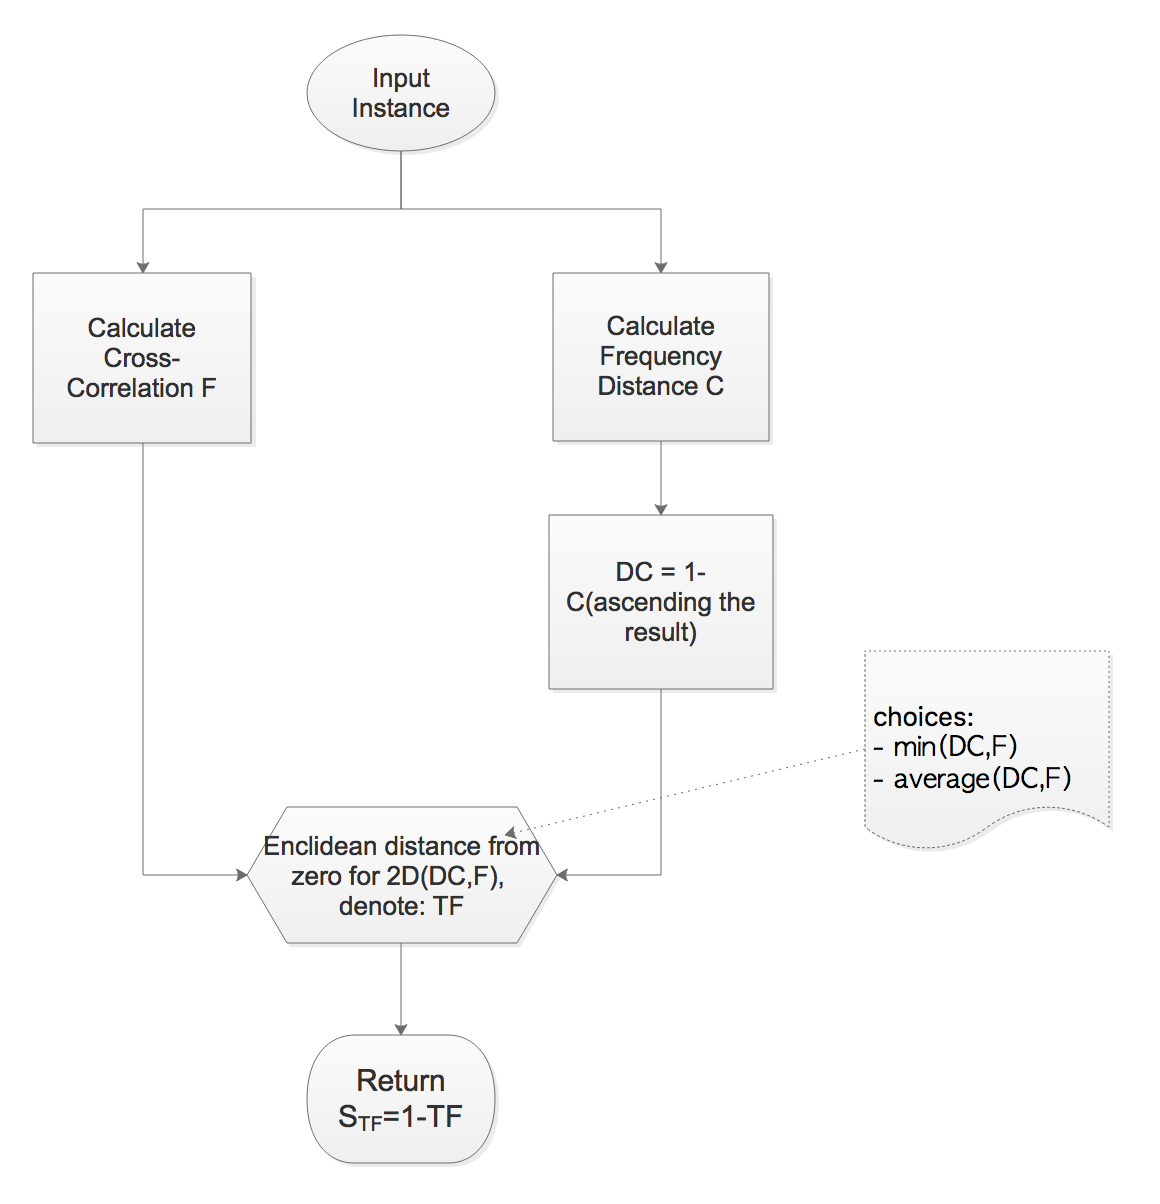
\includegraphics[scale=0.6]{tfClassification.png}
        \caption{Overview of Time Frequency Classification}
        \label{fig:8}
\end{center}
\end{figure} \par
\FloatBarrier

At last, to get a result of decreasing order we return the $S_{TF} = 1-TF$. \\
\newpage

\subsubsection{Typing styles}

The authors categories typing styles in 3 for performance testing: \\

\begin{tabular}{| l | l | }
\hline Style & Features \\
\hline \textbf{Straw Man Approach}: & \tabincell{l}{Typing each letter multiple times using the same finger.\\
- No overlap of keyboard \\
- Approximately the same force\\
- Hit the key from the same angle } \\

\hline \textbf{Hunt and Peck: } & \tabincell{l}{random words typed\\
- Type the letter consecutively different\\
- Hit the key from different angles\\}\\

\hline \textbf{Touch Typing: } & \tabincell{l}{each key has its own designated finger and\\
the rest fingers can possibly touch the key\\
- The keys are hit from different angles\\
- Hand position and finger choice are important\\}\\

\hline
\end{tabular}

\subsection{Fiona}

A.Fiona proposed in 2006 published a empirical study of the acoustic triangulation attack based on a distance-time theory.\\ 

\subsubsection{Hypothesis}

Triangulation is defined as seeking the distance of a point using the concept of triangle, as shown by Figure~\ref{fig:9} below. \\

\begin{figure}[h]
\begin{center}
        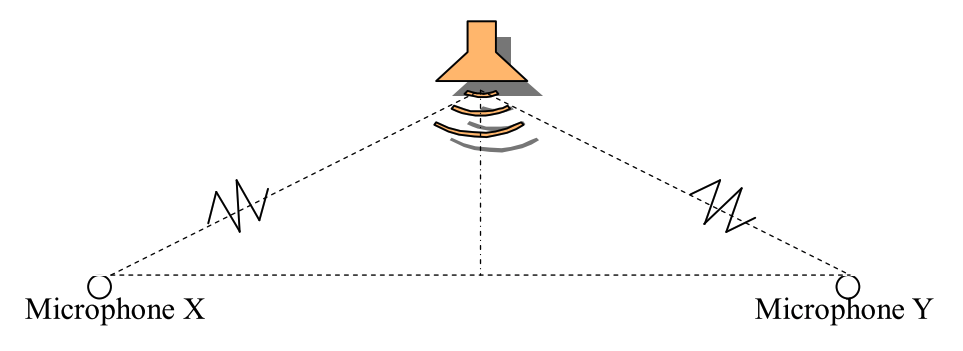
\includegraphics[scale=0.45]{triAng.png}
        \caption{Acoustic Triangulation Description}
        \label{fig:9}
\end{center}
\end{figure} \par
\FloatBarrier

By detecting and measuring the differences in arrival times from two microphones, the location can be easily found. \\

Given that the distance between key i and microphone X be $D_{ix}$ and the one between key i and microphone Y be $D_{iy}$, and the keystroke emits a sound which has a velocity in the air:V.\\

The difference between two microphones can be calculated as follows: \\

time delay of the sound of the key i is $t{i}$:\\

$t_{i}$ =  the time required for the sound wave to reach microphone X - the time required for the sound wave to reach microphone , which is:\\

$t_{i} = D_{ix}/V - D_{iy}/V = (D_{ix}-D_{iy})/V$\\

The hypothesis is that the $t_{i}$ we calculate is unique for each key.\\

\subsubsection{Compare Technologies}

In the study of A.Fiona, 2 approaches is suggested for the comparisons arriving times between microphone X and microphone Y. \\

\textbf{The Maximum Peak Position} captures the maximum peak for each PRESS and RELEASE pair, and compare the time difference between T1-T2 as shown in Figure~\ref{fig:10}\\

\begin{figure}[h]
\begin{center}
        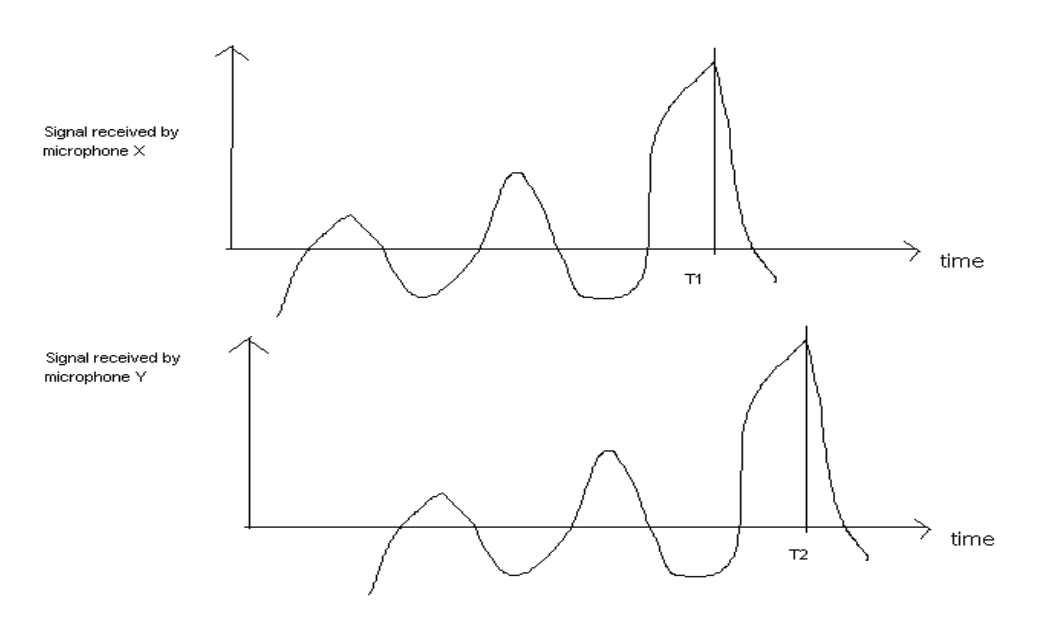
\includegraphics[scale=0.45]{xyPeakComp.png}
        \caption{Maximum Peak Difference}
        \label{fig:10}
\end{center}
\end{figure} \par
\FloatBarrier

Another approach is \textbf{The Cross-Correlation}: consider x(i) and y(i) the digital signals received by Microphone X and Microphone Y respectively. The correlation at delay d is : \\

$r(d) = \frac{\sum\limits_i [(x(i)-mx)*(y(i-d)-my)] }{\sqrt{\sum\limits_i (x(i)-mx)^{2}} \sqrt{\sum\limits_i (y(i-d)-my)^{2}}}$\\

As shown in Figure~\ref{fig:11}, r(d) will be the greatest when x(i) overlaps with y(i-d). In this way, we can find the delay d by constructing the graph r(d) against d.\\

\begin{figure}[h]
\begin{center}
        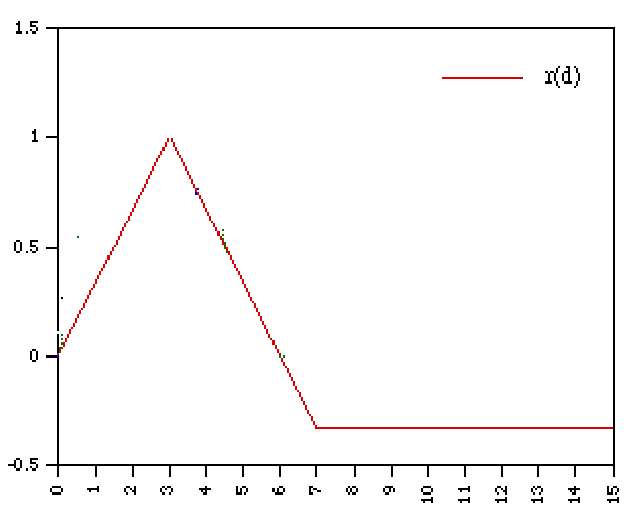
\includegraphics[scale=0.5]{XcorRdd.png}
        \caption{A graph of r(d) against d}
        \label{fig:11}
\end{center}
\end{figure} \par
\FloatBarrier

\subsubsection{Attack Processes Overview}

This type of attack will not require the attacker to have a relatively good understanding in the feature extraction and classification, but simply measuring the time delay between keystrokes. Further more, since no computation in frequency domain is required in the new attack, even the keyboard is designed to produce the same sound, this measurement is still effective in getting the information.\\ 

3 steps are generated for this purpose: \\

\begin{tabular}{| l | l | }
\hline Step & Description \\
\hline \textbf{1. Sound Collection }: & \tabincell{l}{
- Convert analogue sound waves into digital signals\\
- Parameters set in order to keep its original form\\
- Pre-processing  making it more distinguishable } \\
\hline \textbf{2. Signal Analysis }: & \tabincell{l}{
- calculate the arriving time differences between\\
 two microphones\\
- Analysis Methodologies: \\
\qquad - Maximum Peak Position \\
\qquad - Correlation } \\
\hline \textbf{3. Statistical Classification }: & \tabincell{l}{ 
- Neural Networks \\
- HMM (Hidden Markov Models)} \\
\hline
\end{tabular}\\


\section{Experiment Design}

\subsection{Overview of Technologies}

As we summarized in Table~\ref{tab:1}, each approach has its own advantage and defaults. One of the objective of this project is to recreate one of the attack acoustic described there. \\

Since our time is limited, the goal of this experiment is to generate a key press by analyzing the acoustic signal as it was described by Asonov and Agrawal in the 2004. 

\begin{sidewaystable}[h]
\caption{Compare Horizontal Methodologies}
\label{tab:1}
\begin{tabular}{| l | l | l | l | l | l |}
\hline \hline
Procedure & Asonov and Agrawal & Zhuang et al & Berger et al & Halevi and Saxena & Fiona \\
\hline Hypothesis & \tabincell{l}{different sound \\ in different position} &
\tabincell{l}{The input is not\\ random} &
\tabincell{l}{Interval decide position} &
\tabincell{l}{Type style influence\\ the result} &
\tabincell{l}{Distance can be\\ measured by delay} \\
\hline Equipments & 1 Microphone &  1 Microphone & 1 Microphone & 1 Microphone & 2 Microphone \\
\hline \tabincell{l}{Collection sound\\ pre-processing} & No & Yes & No & No & Yes\\
\hline \tabincell{l}{supervised \\ unsupervised} & supervised & unsupervised & unsupervised & ---- & supervised \\
\hline \tabincell{l}{Keystroke recognizing} & Press Peak & \tabincell{l}{start position} & \tabincell{l}{Press and Release} & ---All---- & Maximum Peak \\
\hline \tabincell{l}{Feature \\Extraction} & 
\tabincell{l}{ FFT}&
\tabincell{l}{ FFT and MFCC \\ Cepstrum features} &
\tabincell{l}{ $Sim(K_{1},K_{2})$} & 
\tabincell{l}{FFT and X-Corr} & 
\tabincell{l}{Delay or \\ d from X-Corr} \\
\hline \tabincell{l}{Classification \\ method} &
\tabincell{l}{Neural network \\ classification} &
\tabincell{l}{Neural Network \\ Linear Classification \\Gaussian Mixture} & %newpnn() and clasify() in matlab
\tabincell{l}{Prioritization Algorithm \\ specific} &
\tabincell{l}{Not Specified}&
\tabincell{l}{Neural Network \\ HMM } \\
\hline \tabincell{l}{Linguistic Approach} &
\tabincell{l}{No} &
\tabincell{l}{HMM and \\ Grammar Model}&
\tabincell{l}{Dictionary or Not}&
No &
No \\
\hline Evaluation & No &
\tabincell{l}{HMM and \\ Grammar Model} &
\tabincell{l}{Precision \\and Recall} &
------ & No \\
\hline \tabincell{l}{Feeding Back \\ Training}& No & Yes & No & ------& No \\
\hline
\end{tabular}
\end{sidewaystable}


\subsection{Environment Setup}
In this experiment, we will use the HHKB keyboard as shown in Figure~\ref{fig:12} \\
\begin{figure}[h]
\begin{center}
        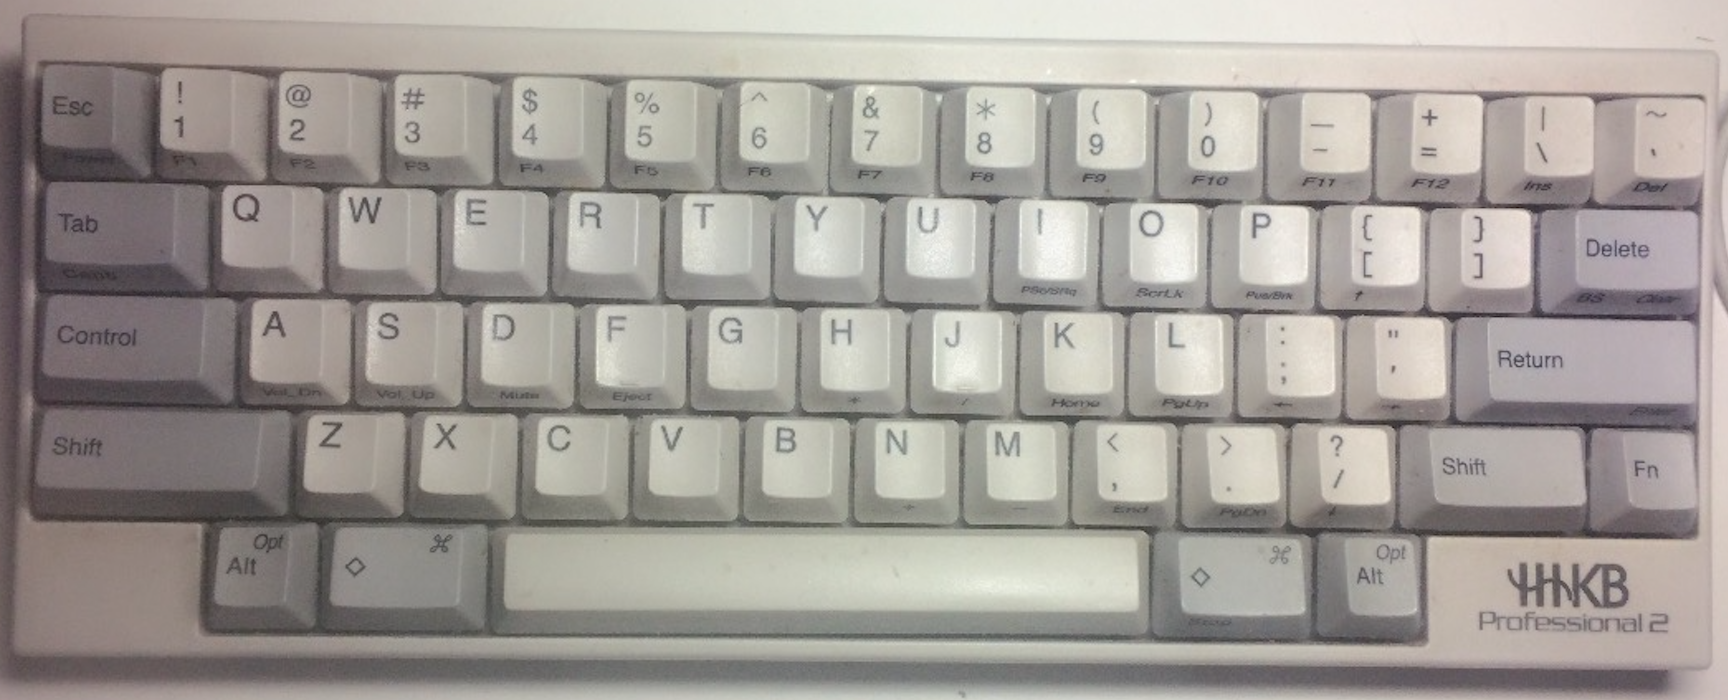
\includegraphics[scale=0.5]{HHKB.png}
        \caption{Keyboard HHKB Pro 2}
        \label{fig:12}
\end{center}
\end{figure} \par
\FloatBarrier

For the system environment we will use : \\

\begin{tabular}{| l | l | }
\hline Env  & Details \\
\hline \textbf{System}: & \tabincell{l}{MacOS Sierra Version 10.12.3\\
Model mi-2014 Retina\\
Processor : 2.6GHz Intel Core i5 \\ 
Memory : 8G } \\

\hline \textbf{Version Mathlab}: & \tabincell{l}{Matlab R2016a 9.0.0.341360 } \\
\hline \textbf{Recording Software}: & \tabincell{l}{Sound Studio Version 4.8.3} \\

\hline
\end{tabular}

\subsection{Experiment Process}
\subsubsection{Record the Signals}
	Make sure that the computer has a microphone which functions well. When we click on the record button of Sound Studio, it will create a recorder object that records on two channel of data 44.1 KHz with 16-bit samples.\\
	
	Once we stopped recording, we will capture the recording as a *.wav file, and save it locally. \\
	
	In the Matlab, we can extract the raw data with the command :\\

	[x,fs]=audioread('q1.wav');\\
	
	Then get one channel from it by extracting one colon from the list: \\
	
	s1 = x(:,1); \\

	We can plot out the figure by these command :\\ 
	
	figure(1);\\
	
	plot(s1);\\

	We will have Figure ~\ref{fig:13} with with we can observe easily the PRESS and RELEASE actions. \\
\begin{figure}[h]
\begin{center}
        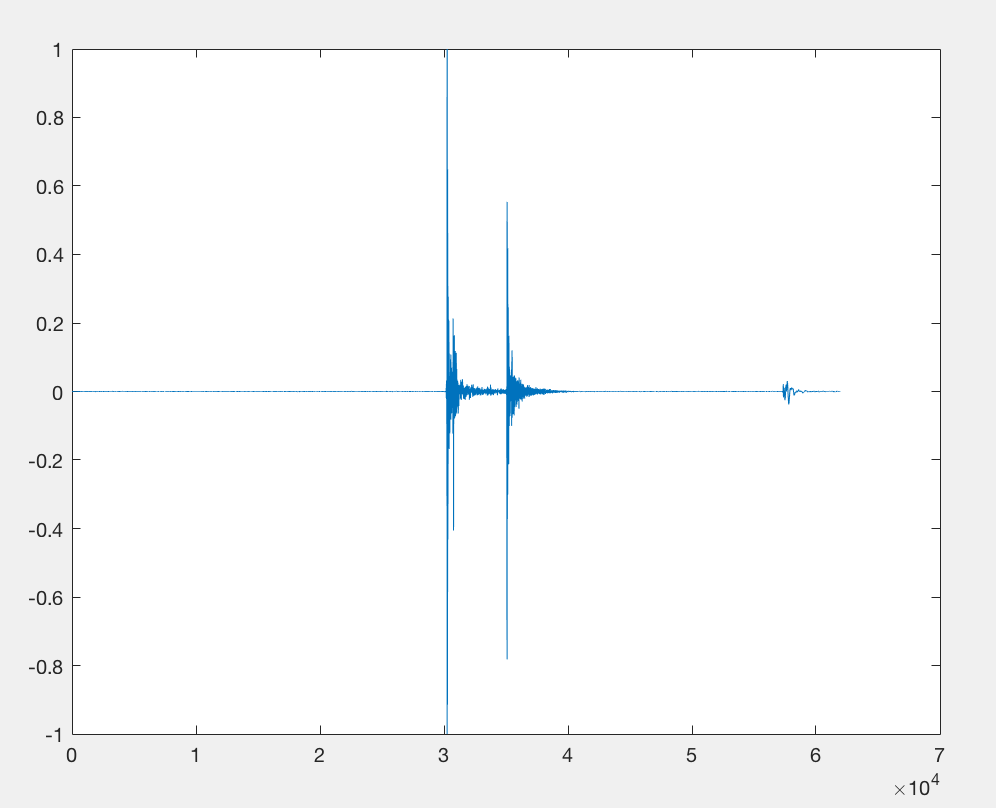
\includegraphics[scale=0.5]{fig13.png}
        \caption{The graph of a single keystroke}
        \label{fig:13}
\end{center}
\end{figure} \par
\FloatBarrier

We should zoom in to get the peak of a press action then extract it from the array by using the command : \\

s1 = s1 (begin: end)\\

\subsubsection{Process the Signals}

Now for each array, we want to do an FFT to find the frequency spectrum for the key press:\\

N=512;\\

Xa = fft(a,N);\\

Xb = fft(b,N);\\




\subsubsection{Classify the Signals}
Using these FFTs, we can create a neural network that can be used to guess key presses. MATLAB has a neural network toolbox that can be used for pattern recognition and classification.\\

X = [Xa Xb]; \\

T = [0 1];\\

net = newpr(X, T, 20); \\ 

The X array is the set of input vectors to the neural net, T is the set of target outputs. X is a 512x2 array with 2 input vectors each with 512 data points. The target array has two values that correspond to the 2 input vectors. A 0 indicates the corresponding input vector is key ‘a’ and a 1 indicates the input vector is for key ‘b’. If you collect more input data – i.e. more recordings of the two keys – we can add them as input vectors to X. The corresponding values will need to be added to the target vector as well. The more inputs we have, the more accurate the neural network.\\

the next step is to train the network.\\

net = train(net, X, T); \\

This, will bring up a new window that shows the neural network training progress as shown in Figure ~\ref{fig:14} \\
\begin{figure}[h]
\begin{center}
        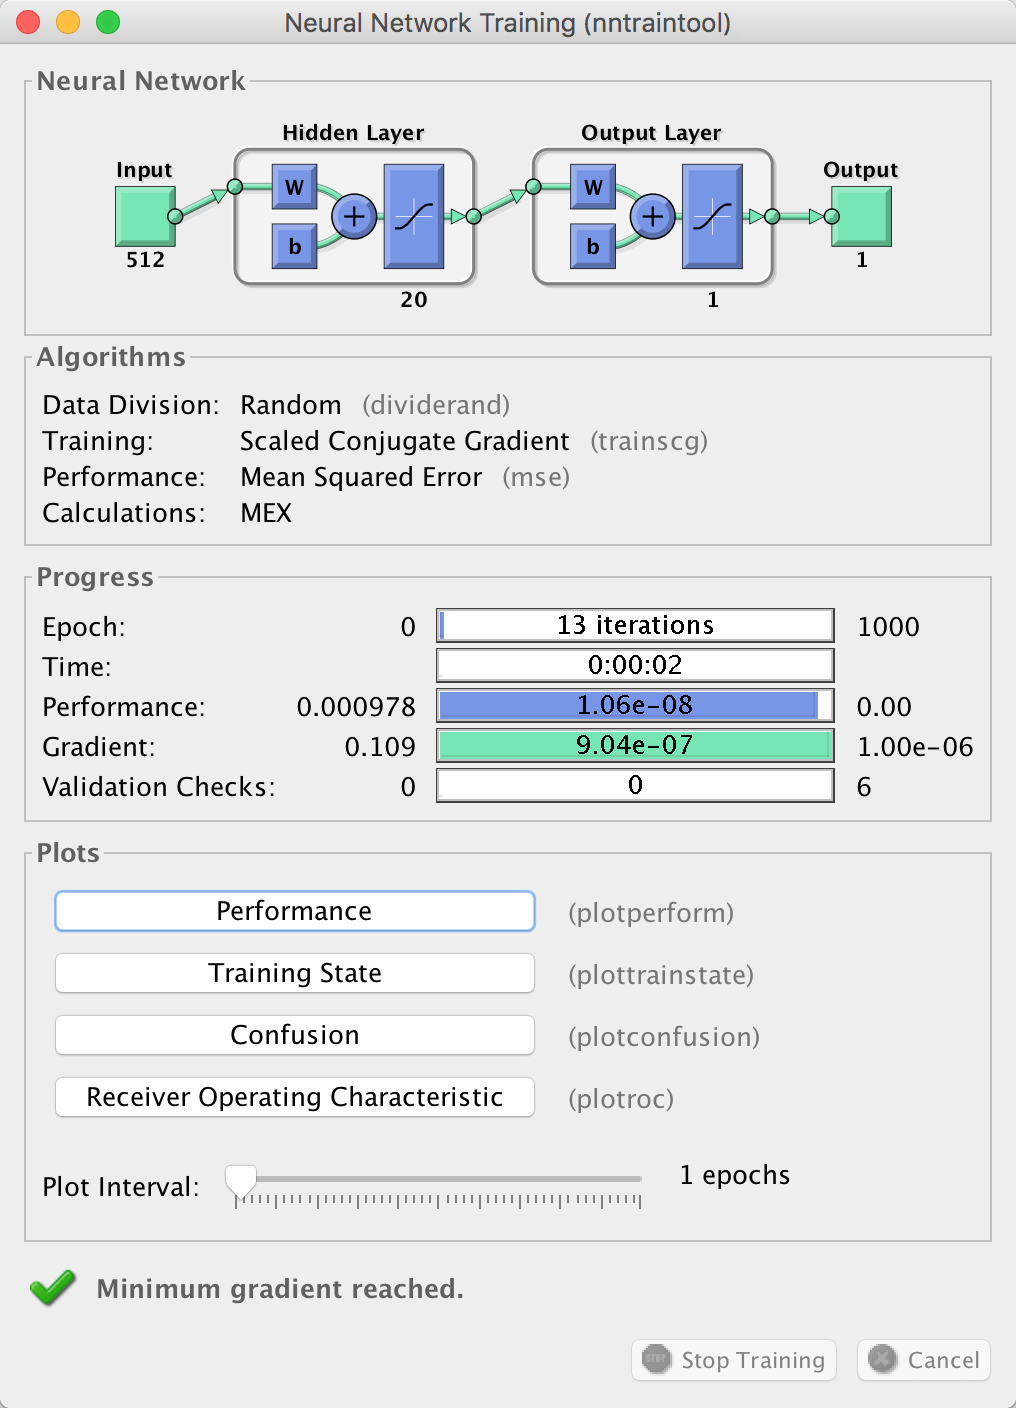
\includegraphics[scale=0.5]{fig14.png}
        \caption{Neutral Classification Window}
        \label{fig:14}
\end{center}
\end{figure} \par
\FloatBarrier

Now that the network has been trained, we can use the neural network to evaluate a new input FFT with the function sim (net, x);\\

A value close to 1 indicates that the key is more probably be a 'b'.\\

As this goes, the rest is to enrich the dataset of this model. 

\section{Conclusion}

We have performed an state of art computing techniques concerning the acoustic side channel  attack and we have performed it on the signal press based on the work of Asonov and Agrawal in the year 2004. \\

But as we limited by the time, I didn't have a static study of the accuracy for the method Asonov and Agrawal, and for the same reason, the time will not allow me to go for all the technologies listed above.  \\

\bibliographystyle{IEEEtran}
\bibliography{biblio}

\end{document}
	
	
